\section{Energy Shaping}
\showtoc

\subsection{Energy Shaping with Control Lyapunov Functions}

\begin{frame}
  \frametitle{Motivation}
  \begin{block}{Main Question}
    Can we use an understanding of energy exchange to improve global stability
    properties of periodic orbits in mechanical systems?
  \end{block}

  \begin{block}{Observations}
    \begin{itemize}
    \item Numerous control design schemes exist for stabilizing mechanical
      systems to periodic orbits.
    \item Some controllers produce good behavior locally but lack robustness.
    \item Periodic orbits have associated energy functions with level sets which
      are invariant under the orbits.
    \end{itemize}
  \end{block}
\end{frame}

\begin{frame}[t]
  \frametitle{Overview}
  \only<1>{
    \begin{block}{Setup}
      Consider the control system 
      \begin{align*}
        \dx = \xf(\x) + \xg(\x) \, \uu(\x).
      \end{align*}
      Assume there exists a control law ${\bar \uu}\arx$ which creates a limit
      cycle in the closed-loop dynamics,
      \begin{align*}
        {\bar \xf}\arx = \xf\arx + \xg\arx \, {\bar \uu}\arx.
      \end{align*}
      Also assume there exists an energy function $E_{c} : T\X \to \R$ which is
      conserved, i.e., $E_{c}\arx \equiv E_{0}$, on the limit cycle.
    \end{block}
  }

  \only<2>{
    \begin{block}{Main Idea}
      Add robustness to a periodic behavior by imposing convergence on an energy
      function to a level set which is known to be invariant under the system dynamics.
    \end{block}
    
    \begin{block}{Control Objective}
      Choose control input $\mu\arx$ such that $\| \mu\arx - {\bar \uu}\arx \|$ is minimized and $E_{c}\arxt \to E_0$ as $t \to \infty$.
    \end{block}

    \begin{block}{Exponential Convergence}
      To achieve exponential stabilization, $E_{c}(x(t))$ should satifisy
      \begin{align*}
        E_{c}\arxt \leq E_{c}\arxzero e^{-\beta t} \mbox{ for } t \geq 0, \beta > 0.
      \end{align*}
    \end{block}
  }
\end{frame}

\begin{frame}
  \frametitle{Control Lyapunov Functions}
  A \blue{control Lyapunov function} $\V : \X \to \R$ which satisfies
  \begin{align*}
    &c_{1} \nx^{2} \leq \V\arx \leq c_{2} \nx^{2},\\
    &\inf_{\uu \in \U} \Lie{\xf}\V\arx + \Lie{\xg}\V\arx \, \uu + c_{3} \V\arx \leq 0
  \end{align*}
  for $c_{1}, c_{2}, c_{3} > 0$ exhibits exponential convergence. If the above
  are satisfied, then it is also true that
  \begin{align*}
    \left\| \pd{\V\arx}{\x} \right\| \leq c_{4} \nx.
  \end{align*}
\end{frame}


\begin{frame}
  \frametitle{Rapidly Exponentially Stabilizing Control Lyapunov Functions}
  A \blue{rapidly exponentially stability control Lyapunov function (RES--CLF)}
  $\Ve : \X \to \Rnn$ satisfies
  \begin{align*}
    &c_{1} \nx^{2} \leq \Ve\arx \leq \frac{c_{2}}{\resclfparam^{2}} \nx^{2},\\
    &\inf_{\uu \in \U} \Lie{\xf}\Ve\arx + \Lie{\xg}\Ve\arx \, \uu +
    \frac{c_{3}}{\resclfparam} \Ve\arx \leq 0
  \end{align*}
  for $c_{1}, c_{2}, c_{3} > 0$ exhibits exponential convergence. If the above
  are satisfied, then it is also true that
  \begin{align*}
    \left\| \pd{\Ve\arx}{\x} \right\| \leq c_{4} \nx.
  \end{align*}
\end{frame}

\begin{frame}
  \frametitle{Energy Shaping}
  Consider a conserved energy function $E_{c}\arx$ and define a candidate
  control Lyapunov function:
  \begin{align*}
    V\arx = \frac{1}{2} \left(\Ec\arx - \Eref\right).
  \end{align*}
  For an exponentially stabilizing CLF, we seek $\mu\arx$ such that
  \begin{align*}
    \Lie{\xf} V\arx + \Lie{\xg} \V\arx \, \mu\arx + \epsilon \V\arx &\leq 0.
  \end{align*}
  % We can relax this condition by augmenting the optimization space with $\delta \in \R$ and requiring
  %\begin{align*}
  %  2 \eta\arx \left(\Lie{\xf} \eta\arx + \Lie{\xg} \eta\arx \, \mu\arx \right) + \epsilon \eta^{2}\arx \leq \delta\arx.
  %\end{align*}
\end{frame}

\begin{frame}[t]
  \frametitle{Quadratic Program Formulation}
  The linear form of the CLF condition suggests
  \begin{align}
    \nonumber
    \mueps\arx = \argmin_{\uu \in \R^{n}}  \, & \uu^T \uu\\
    \label{eq:clf} \tag{clf}
    \mbox{s.t. } & \Aclf\arx \, \uu \leq \bclf\arx%\\
    %\label{lim} \tag{lim}
    %& \Alim v \leq \blim
  \end{align}
  where \eqref{eq:clf} imposes the control Lyapunov function. To encode the dynamics of the system, select
  \begin{align*}
    \Aclf = \Lie{\xg}\Ve\arx, && \bclf = -\Lie{\xf}\Ve\arx - \frac{c_{3}}{\resclfparam} \Ve\arx.
  \end{align*}
\end{frame}

\begin{frame}
  \frametitle{Closed-Loop Hybrid System}
  Applying the energy shaping controller gives the closed-loop hybrid system
  \begin{align*}
    \HSeps = \left\{
      \begin{array}{l l}
        \dx = \xf\arx + \xg\arx \, \mueps\arx, & \x \in \D \setminus \S,\\
        \xp = \Delta(\xm), & \x \in \S.
      \end{array}\right.
  \end{align*}
  This is called the \blue{shaped system}. It has a periodic orbit, $\orbit$,
  which is identical to that of the unshaped system, $\HS$.
\end{frame}

\subsection{Energy Shaping Theorem}

\begin{frame}
  \frametitle{Main Theorem}

  \begin{theorem}[Energy Shaping]
    Given an exponentially-stable cycle in a hybrid system, application
    of the energy shaping controller results in the closed-loop hybrid system
    \begin{align*}
      \HS_{\resclfparam} = \left\{
      \begin{array}{l l}
        \dx = \xf\arx + \xg\arx \, \mueps\arx, & \x \in \D \setminus \S,\\
        \xp = \Delta(\xm), & \x \in \S,
      \end{array}\right.
  \end{align*}
  which is exponentially stable about the hybrid periodic orbit $\orbit$ for
  large enough $\resclfparam$.
  
  \end{theorem}
\end{frame}

\begin{frame}
  \frametitle{Zero Dynamics Formulation}
  Construct a change of coordinates, splitting up the system into two sets of coordinates:
  \begin{align*}
    \dot \zdx &= f\argsxz + g\argsxz \, \uu,\\
    \dot \zdz &= q\argsxz + w\argsxz \, \uu.
  \end{align*}
  The vector fields $f$, $g$, $q$, and $w$ are assumed to be locally Lipschitz
  continuous. For simplicity, define
  \begin{align*}
    \bigF\argsxz = \left(\begin{array}{c}
        f\argsxz\\
        q\argsxz
      \end{array}\right),&&
    \bigG \argsxz = \left(\begin{array}{c}
        g\argsxz\\
        w\argsxz
      \end{array}\right).
  \end{align*}
\end{frame}

\begin{frame}
  \frametitle{Energy-Based Coordinate Change}
  For mechanical systems with coordinates $\x = \argsqdq \in T\Q$, construct the transformation $\xform\argsqdq := \argsxz$ where
  \begin{align*}
    \zdx &= \Ec\argsqdq - \Eref,\\
    \zdz &= \xrem,
  \end{align*}
  where $n$ is the size of the configuration space, $\Q$. The fixed point of the
  hybrid system is chosen to occur at $\argsxz = \xzst$ such that $\Delta\xzst =
  \argszero$.
\end{frame}

\begin{frame}
  \frametitle{Validity of Transformation}
  The coordinate change $\xform\argsqdq$ is valid if it is locally diffeomorphic around the orbit
  $\orbit$, i.e., if
  \begin{align}
    \pd{\xform(\q, \dq)}{(\q, \dq)} =
    \left(\begin{array}{c c}
        I_{2n-1} & \boldzero_{2n-1 \times 1}\\
        \pd{E(\q, \dq)}{\xrem} & \pd{E(\q, \dq)}{\dq_{n}}
      \end{array}\right)
  \end{align}
  % 
  has full rank, which occurs when
  \begin{align*}
    \det\left(\pd{\xform\argsqdq}{\argsqdq}\right) = \pd{E(\q, \dq)}{\dq_{n}} \ne 0.
  \end{align*}
\end{frame}

\begin{frame}
  \frametitle{Flows of Continuous Dynamical Systems}
  Recall that the flow of an ODE expressed in the variables $\argsxz$ is given
  by
  \begin{align*}
    \flowt\argsxz = \int_{0}^{t} \left[ \bigF\argsxztau + \bigG\argsxztau \,
      \uu\argsxztau \right] \, d\tau
  \end{align*}
  for some feedback control law $\uu : \zdX \times \zdZ \to \U$. For some stable
  tube $\stabletube$ around the orbit $\orbit$, it holds that the vector fields are bounded:
  \begin{align*}
    \supF & := \sup \left\{ \left\| \bigF\argsxz \right\| : \argsxz \in
      \stabletube \right\},\\
    \lambdamaxG &:= \sup \left\{\lambdamax\bigG\argsxz : \argsxz \in \stabletube
    \right\},\\
    \lambdaminG &:= \inf \left\{\lambdamin\bigG\argsxz : \argsxz \in \stabletube
    \right\}.
  \end{align*}
\end{frame}


\begin{frame}
  \frametitle{Definition of the \Poincare{} map}
  \only<1> {
    The \blue{\Poincare{} first return map} takes a point on the guard, applies
    the reset map and then integrates forward until the guard is reached
    again. For the shaped system, $\Pe : \S \to \S$, is defined by
    \begin{align*}
      \Pe\argsxz = \floweps_{\TIeDelta}\argsDeltaxz,
    \end{align*}
    where $\TIe : \zdX \times \zdZ \to \Rnn$ is the \tti{} function which is
    defined by
    \begin{align*}
      \TIe\argsxz = \inf \{ t \geq 0 : h(\flowepst\argsxz) \}
    \end{align*}
    and is locally Lipschitz continuous by the implicit function theorem.
  }

  \only<2> {
    \begin{figure}
      \centering
      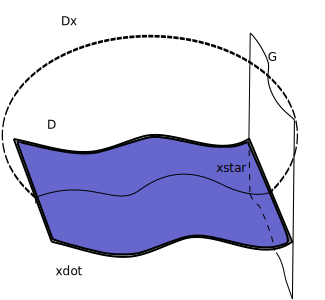
\includegraphics[height=.5\textheight]{hybrid_periodic_orbit}
    \end{figure}
  }
\end{frame}

\subsection{Sketch of Proof}

\begin{frame}
  \frametitle{Equivalence of Hybrid Periodic Orbits}
  \begin{theorem}
    Applying the energy shaping controller to the hybrid control system $\HCS$
    results in the closed-loop hybrid system $\HSeps$ that demonstrates a
    periodic orbit which is identical to the unshaped system $\HS$.
  \end{theorem}
  \begin{proof}
    The energy of states $\xo \in \orbit$ is a constant,
    $\E(\xo) \equiv \Eref$. By the choice of Lyapunov function,
    $Ve(\xo) \equiv 0$. In addition, $\dVe(\xo) \equiv 0$ since
    the system is conservative. And since the solution to the optimization
    problem has cost $\uu(\xo)^{T} \uu(\xo) \equiv 0$, the
    control effort is also zero. Hence the orbits are equivalent.
    \end{proof}
\end{frame}

\begin{frame}
  \frametitle{Boundedness of \TtI{} function}
  \begin{lemma}[Boundedness of \TtI{}]
    For the hybrid systems $\HS$ and $\HSeps$,
    \begin{eqnarray}
      \nonumber
      &| \TIe(\Deltaxz) - \TI(\Deltaxz) | \leq \ATIe \nzdxzst,\\
      &\| \Pe\argsxz - \P\argsxz \| \leq \Ae \nzdxzst,
    \end{eqnarray}
    where $\limeps \ATIe = 0$ and $\limeps\Ae = 0$.
  \end{lemma}
\end{frame}

\begin{frame}
  \frametitle{Proof of Energy Shaping Theorem}
  \only<1> {
    Define a composite Lyapunov function,
    \begin{align*}
      \VP\argsxz = \Vn\argsxz + \sigma \Vex(\zdx),
    \end{align*}
    where
    \begin{itemize}
    \item $\Vn$ : Lyapunov function guaranteed by stability of the nominal system
      (converse Lyapunov theorem)
    \item $\Vex$ : Lyapunov function for energy shaping control law
    \end{itemize}
    with scaling parameter $\sigma$. This is a discrete Lyapunov function that
    is valid on the guard.
  }
  
  \only<2> {
    Exponential stability of the hybrid system $\HS$ is guaranteed by the
    discrete Lyapunov theorem if
    \begin{eqnarray*}
      &r_{1} \nzdxzst^{2} \leq \VP\argsxz \leq r_{2} \nzdxzst^{2}\\
      &\VP(\Pe\argsxz) - \VP\argsxz \leq r_{3} \nzdxzst^{2}
    \end{eqnarray*}
    for some $r_{1}, r_{2}, r_{3} \in \Rnn$.
  }
\end{frame}
